%----------------------------------------------------------------------------
\chapter{Method}
\label{chap:method}
%----------------------------------------------------------------------------

The model generates a target paper's abstract from embeddings of its references, without receiving the target's own title or abstract as input (\autoref{fig:method-overview}). First, a GNN aggregates the reference embeddings to estimate the embedding that would be obtained from the target's title and abstract (\autoref{sec:embeddings}). I call this vector the GNN estimate. This estimate is then passed to the reader, which consists of a prefix adapter and a language model adapted with LoRA. The adapter converts the estimate into prefixes through which the language model receives information about the target and generates its abstract.

The GNN estimator and reader are initially trained separately and then fine-tuned together to generate the target abstracts. During joint fine-tuning, the GNN, prefix adapter and LoRA parameters are trainable, while the original language-model weights remain frozen. The reader can also receive alternative vectors, such as the reference mean (\autoref{sec:reference-information}), allowing the effect of the learned GNN estimate to be examined.

\begin{figure}[!ht]
  \centering
  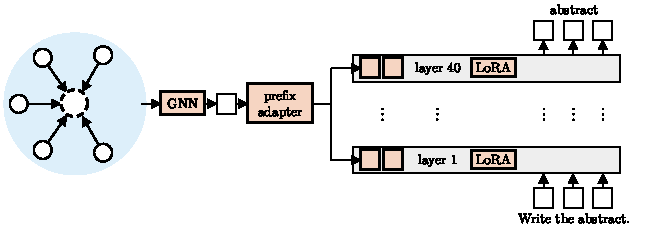
\includegraphics{../diagrams/figures/method/method_overview.pdf}
  \caption{Overview of the model. The references of a target paper (white circles in the blue 1-hop region) pass their embeddings to the target (dashed outline), whose own embedding is not an input; arrows show the direction of information flow. The GNN aggregates them into one vector, the GNN estimate. The prefix adapter maps this vector to key and value prefixes (the two squares at the left of each layer) for every one of the 40 layers of the language model, which is fine-tuned with LoRA. The prompt is the same for every paper; only its last sentence is shown. Red: trainable; grey: frozen.}
  \label{fig:method-overview}
\end{figure}

%----------------------------------------------------------------------------
\section{The GNN estimator}
\label{sec:gnn-estimator}
%----------------------------------------------------------------------------

The GNN estimator receives a target paper together with all of its recorded references, each represented by its embedding (\autoref{sec:embeddings}). The edges point from each reference to the target (\autoref{sec:model-graph}), so the target aggregates information only from the papers it cites. Because the target's own embedding is the vector to be estimated, it cannot also be an input. Before message passing, I therefore replace the target's feature vector with a learned vector $\mathbf{m} \in \mathbb{R}^{1024}$, which I call the \texttt{[MASK]} vector. The same vector is used for every target, so it carries no information about any particular paper; it only marks the node whose embedding is unknown.

Each attention head forms a weighted sum of the reference embeddings after applying a learned transformation, with the attention weights computed as in \autoref{sec:gatv2}. The target also participates through its shared \texttt{[MASK]} vector: the layer adds a self-loop to every node, so the target attends to its own \texttt{[MASK]} vector as well as to its references. This self-loop is part of the attention layer and is not one of the citation self-loops removed in \autoref{sec:model-graph}: it carries the \texttt{[MASK]} vector, not the target's embedding. With $\mathbf{h}_v = \mathbf{m}$ for the target $v$ and $\mathbf{h}_w = \mathbf{x}_w$ for a reference $w$, the output of head $k$ is
\begin{align}
  \mathbf{z}^{(k)}_v = \sum_{w \in \mathcal{N}(v) \cup \{v\}} \alpha^{(k)}_{vw} \mathbf{W}^{(k)}_2 \mathbf{h}_w,
  \label{eq:gnn-head}
\end{align}
where the attention weights $\alpha^{(k)}_{vw}$ are computed by \autoref{eq:gatv2-score} and \eqref{eq:gatv2-softmax} from the head's own parameters $\mathbf{W}^{(k)}_1, \mathbf{W}^{(k)}_2 \in \mathbb{R}^{256 \times 1024}$ and $\mathbf{a}^{(k)} \in \mathbb{R}^{256}$. Each head reads the same complete 1024-dimensional input vectors and produces a 256-dimensional output.

The estimator uses one GATv2 layer with $K = 4$ such heads, whose outputs are concatenated~\cite{velickovic2018graph} (\autoref{fig:gnn-estimator}):
\begin{align}
  \mathbf{h}'_v = \big[\mathbf{z}^{(1)}_v \,\Vert\, \mathbf{z}^{(2)}_v \,\Vert\, \mathbf{z}^{(3)}_v \,\Vert\, \mathbf{z}^{(4)}_v\big] + \mathbf{b},
  \label{eq:gnn-heads}
\end{align}
where $\Vert$ denotes concatenation and $\mathbf{b}$ is a learned bias. The inputs are not split into four pieces: four learned transformations operate on the same inputs, and their outputs are concatenated into a vector of 1024 values, the dimension of the embeddings. Because each head has its own parameters, different heads can assign different weights to the same references. Unlike in \autoref{eq:gatv2-output}, no nonlinearity is applied to the output. With a single layer, the output depends only on the direct references of the target, not on the papers that they cite in turn.

\begin{figure}[!ht]
  \centering
  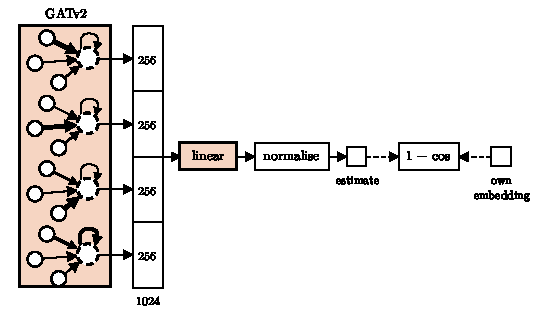
\includegraphics{../diagrams/figures/method/gnn_estimator.pdf}
  \caption{The GNN estimator. Inside the GATv2 layer, the same neighbourhood is drawn once for each of the four attention heads: the references send their embeddings to the target (dashed outline), whose embedding is replaced by the learned \texttt{[MASK]} vector; the self-loop lets the target attend to this vector. The width of each arrow indicates the attention weight that the head assigns to it; the widths are illustrative. Each head outputs 256 values, and the four outputs are concatenated into a vector of 1024 values, which passes through a linear layer and is normalised to unit length, giving the GNN estimate. The dashed branch provides embedding supervision during training: the loss is one minus the cosine similarity between the estimate and the target's own embedding. Red: trainable.}
  \label{fig:gnn-estimator}
\end{figure}

A linear layer maps $\mathbf{h}'_v$ to the final output, which is normalised to unit length:
\begin{align}
  \hat{\mathbf{x}}_v = \frac{\mathbf{W}_o \mathbf{h}'_v + \mathbf{b}_o}{\lVert \mathbf{W}_o \mathbf{h}'_v + \mathbf{b}_o \rVert}, \qquad \mathbf{W}_o \in \mathbb{R}^{1024 \times 1024}.
  \label{eq:gnn-output}
\end{align}
The vector $\hat{\mathbf{x}}_v$ is the GNN estimate. The normalisation gives it the same length as the embeddings, which are the vectors the reader receives during its own training.

During separate training of the GNN estimator, I minimise
\begin{align}
  \mathcal{L}_{\cos} = 1 - \cos(\hat{\mathbf{x}}_v, \mathbf{x}_v),
  \label{eq:cos-loss}
\end{align}
averaged over the training targets, so that the estimate points in the same direction as the target's own embedding $\mathbf{x}_v$. The objective is defined in the embedding space, so the estimator can be trained without the language model, and its quality can be measured with the same cosine similarity as in \autoref{sec:reference-information}. During separate estimator training, the target's embedding provides supervision; it is not part of the estimator's input. In the final joint training stage, this cosine loss is combined with the abstract-generation loss, allowing the estimator to receive supervision from both objectives (\autoref{sec:training}).

As a parameter-free baseline, I average the embeddings of the same references and normalise the resulting vector to unit length. Unlike the GNN estimator, this reference mean (\autoref{sec:reference-information}) applies neither learned weighting nor learned transformations.

%----------------------------------------------------------------------------
\section{The prefix adapter}
\label{sec:prefix-adapter}
%----------------------------------------------------------------------------

The prefix adapter turns the GNN estimate into a prefix for the language model in the sense of prefix tuning (\autoref{sec:prefix-tuning}): key and value vectors that precede the prompt in every layer (\autoref{eq:prefix}). Unlike in prefix tuning, the prefix is not a fixed set of parameters but is computed separately for each paper. Its shape is determined by the language model. The reader uses Qwen3-14B~\cite{yang2025qwen3}, which has 40 Transformer layers and uses GQA (\autoref{sec:kv-cache}): the 40 query heads of a layer share 8 key--value heads~\cite{yang2025qwen3}, each of dimension 128. At each layer, the adapter supplies 32 prefix positions. Each position needs a 128-dimensional key and value for each of the eight key--value heads. The adapter produces these prefixes separately for all 40 layers, so its output has the shape
\[
  40 \times 2 \times 8 \times 32 \times 128,
\]
where the factors are, in order, the layers, the key and value, the heads, the positions and the head dimension; in total, 2,621,440 numbers. All shapes in this section are for a single paper, with the batch dimension omitted.

A direct mapping from the 1024-dimensional input to the complete prefix, for example a separate linear map for the keys and for the values of each layer, would require approximately 2.69 billion parameters, about 18\% of the 14.8 billion parameters of Qwen3-14B itself. The large output makes such a direct projection expensive. The factorised adapter described below reduces this to approximately 32.1 million parameters. The calculation of these numbers is given in \autoref{app:parameters}.

Instead of learning a separate large mapping for every layer, I first compute a compact code for each layer's keys and values. Two shared decoders then expand these codes into the required prefixes (\autoref{fig:prefix-adapter}). A code is a short vector computed by a learned projection: the codes are computed for each paper, while the parameters of the decoders are shared by all layers. The adapter has three components. The trunk, a linear layer $1024 \rightarrow 1024$ followed by a GELU activation and layer normalisation, transforms the GNN estimate into a shared intermediate representation. The code projection, a single linear layer, maps this representation to 15,360 values, which are sliced into a separate 192-dimensional code for each layer and for each of the key and value roles, 80 codes in total. The two decoders, one for keys and one for values, each expand a code into the $8 \times 32 \times 128$ numbers of one layer's key or value prefix. Because each decoder is shared by all 40 layers, the large output dimension is paid for twice rather than 80 times. Keys and values have separate decoders because they play different roles in attention: the keys determine which positions a token attends to, and the values carry the information that is read from them.

\begin{figure}[!ht]
  \centering
  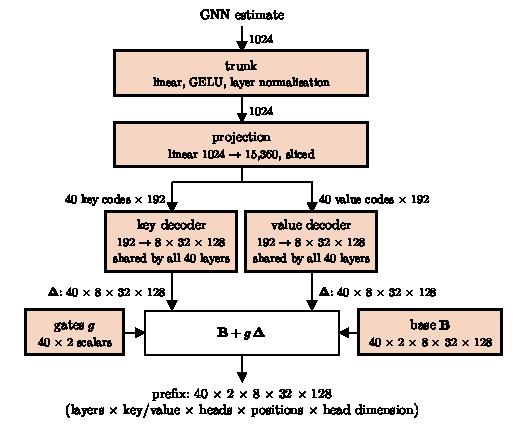
\includegraphics{../diagrams/figures/method/prefix_adapter.pdf}
  \caption{The prefix adapter, with the shape of each intermediate result. The GNN estimate passes through the trunk and one projection, whose 15,360 outputs are sliced into 80 codes of 192 values: one key code and one value code for each of the 40 layers. The key decoder maps each key code, and the value decoder each value code, to 8 heads $\times$ 32 positions $\times$ 128 numbers; each decoder is shared by all 40 layers. The decoder outputs $\boldsymbol{\Delta}$ are scaled by the gates $g$, one per layer and role, and added to the learned base prefix $\mathbf{B}$ (\autoref{eq:prefix-gate}), giving the key and value prefixes of all 40 layers. Red: trainable.}
  \label{fig:prefix-adapter}
\end{figure}

The decoders produce the paper-specific part of the prefix. For layer $\ell$ and role $r \in \{K, V\}$, the full prefix is
\begin{align}
  \mathbf{P}^r_\ell = \mathbf{B}^r_\ell + g^r_\ell \, \boldsymbol{\Delta}^r_\ell,
  \label{eq:prefix-gate}
\end{align}
where $\boldsymbol{\Delta}^r_\ell$ is the decoder output, $\mathbf{B}^r_\ell$ is a learned base prefix and $g^r_\ell$ is a learned scalar gate. The base prefix supplies a learned component common to all papers; it is a prefix in the original sense of prefix tuning and is initialised with small random values (standard deviation 0.02). The 80 gates scale the paper-specific contribution separately for each layer's keys and values. They are initialised to zero and are not restricted in sign or size. At the start of training, the prefix is therefore the same for every paper, and training begins as plain prefix tuning. Initialising the gates to zero initially blocks the paper-specific branch from affecting the prefix. The gates can nevertheless receive gradients and move away from zero, allowing that branch to begin learning. After training, setting the gates to zero removes the paper-specific contribution while retaining the learned base prefix.

The generated prefixes are inserted directly into the language model's key--value cache. They occupy positions 0--31, and the textual prompt starts at position 32, consistently during training and generation.

%----------------------------------------------------------------------------
\section{The reader}
\label{sec:reader}
%----------------------------------------------------------------------------

The reader turns the GNN estimate into an abstract. It consists of the prefix adapter of \autoref{sec:prefix-adapter} and the language model Qwen3-14B~\cite{yang2025qwen3}, adapted with LoRA (\autoref{sec:lora}). During separate reader training, the language-model weights remain frozen, while the prefix adapter and LoRA matrices are updated.

The prefix and LoRA have separate roles. The prefix is the only input that differs between papers: it is computed from the paper's vector. The LoRA parameters, in contrast, are shared across papers and remain fixed during generation. The adapter supplies keys and values directly, rather than obtaining them from the language model's token projections. The prefix supplies paper-specific information, while LoRA adapts the model's processing of that information. Training the adapter and LoRA together allows the supplied representations and the model's response to them to adapt jointly. Their individual contributions are examined in \autoref{chap:ablations}.

I apply LoRA with rank $r = 16$, scaling $\alpha = 32$ (\autoref{eq:lora}) and dropout 0.05 to the query and value projections of all 40 layers. The prefix is inserted as finished keys and values, so the key and value projections of the model never act on it; LoRA changes only the computations for the prompt and abstract tokens. Adapting the query projection changes how tokens attend to the prefix and to other tokens. Adapting the value projection changes the information carried by token values. In later layers, those token states can already contain information obtained from prefixes in earlier layers. \autoref{fig:lora-prefix} shows where LoRA and the prefix act within one attention head.

\begin{figure}[!ht]
  \centering
  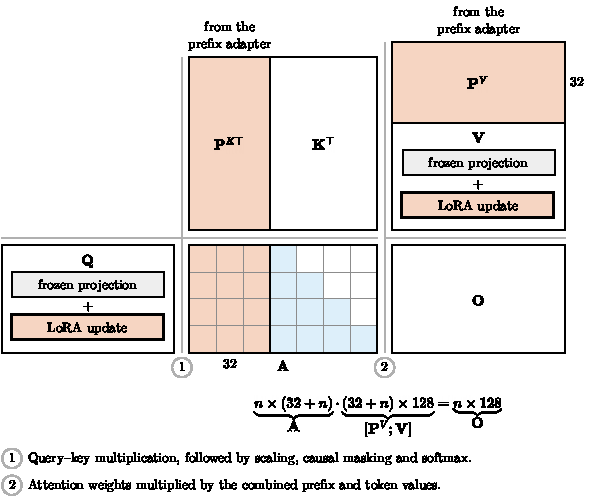
\includegraphics{../diagrams/figures/method/lora_prefix.pdf}
  \caption{Where LoRA and the prefix act in one attention head (one query head and its associated key--value head; schematic). The token queries and values are produced by frozen projections with additive LoRA updates, shared by all papers. The prefix $\mathbf{P}^K$, $\mathbf{P}^V$ is computed for each paper by the prefix adapter and adds 32 positions before the $n$ prompt and abstract positions. In $\mathbf{A}$, red columns are prefix positions and white cells masked future positions. The prefix adds key and value positions, but no query positions. The output therefore retains one 128-dimensional vector per token, as in attention without a prefix. Positional transformations and normalisation are omitted.}
  \label{fig:lora-prefix}
\end{figure}

The textual input is a fixed prompt, identical for every paper, in Qwen3's chat format with the model's reasoning (``thinking'') mode disabled; it is 241 tokens long. No titles or reference abstracts are inserted into this prompt; the paper-specific information arrives through the prefix. The system message asks for an abstract that covers the paper's problem, the prior work it builds on, its approach and its evaluation. Selected excerpts are shown below.

\begin{center}
\fbox{\begin{minipage}{0.9\textwidth}
\textit{Selected excerpts from the fixed prompt; omissions marked [\ldots]}

\textbf{System:}

``The context you have been given encodes the reference list of one paper, whose own abstract is missing.''

[\ldots]

``Where the context leaves the paper's specific contribution undetermined, state what it does determine about its problem and approach, and stop there [\ldots]''

``Write plain prose of 150-180 words, with no markup, mathematical notation or headings.''

``Output ONLY the abstract text.''

\textbf{User:}

``Write the abstract.''
\end{minipage}}
\end{center}

The requested word count is an instruction to the model, not a guarantee about the length of the generated text. The complete prompt is given in \textcolor{red}{[TODO: reference to the appendix with the full prompt]}.

The reader is trained with the next-token cross-entropy of \autoref{eq:lm-loss}. The context consists of the prefix and the prompt, and the target sequence is the paper's abstract, cleaned as described in \autoref{sec:cleaning}. The loss is computed only for the abstract tokens; prompt tokens remain visible as context but do not contribute directly to the loss. Although the original language-model weights are not updated, gradients are propagated through its computations to train the prefix adapter and LoRA parameters.

%----------------------------------------------------------------------------
\section{Model size}
\label{sec:model-size}
%----------------------------------------------------------------------------

\autoref{tab:model-size} lists the number of parameters in each component of the model. The trainable components together have 45.7 million parameters, about 0.3\% of the 14.8 billion parameters of Qwen3-14B, which remains frozen. The calculation for each component is given in \autoref{app:parameters}.

\begin{table}[!ht]
  \centering
  \begin{tabular}{@{}lr@{}}
    \toprule
    component & parameters (millions) \\
    \midrule
    GNN estimator & 3.2 \\
    prefix adapter & 32.1 \\
    LoRA & 10.5 \\
    Qwen3-14B (frozen) & 14,768.3 \\
    \midrule
    all trainable components & 45.7 \\
    \bottomrule
  \end{tabular}
  \caption{Parameters of the model components. LoRA has rank 16 and is applied to the query and value projections of all 40 layers. The exact counts are calculated in \autoref{app:parameters}.}
  \label{tab:model-size}
\end{table}

%----------------------------------------------------------------------------
\section{Decoding}
\label{sec:decoding-method}
%----------------------------------------------------------------------------

All abstracts are generated with greedy decoding (\autoref{sec:decoding}), with the same settings for every input variant compared in \autoref{chap:evaluation}. Generation stops when the model produces an end-of-sequence token or reaches the limit of 320 new tokens. Greedy decoding introduces no random token sampling, so the comparisons are not affected by variation from sampling. I set the generation limit to 320 new tokens as a practical compromise between allowing sufficiently long abstracts and bounding generation time. Under the Qwen3 tokenizer, the cleaned training abstracts have a median length of 191 tokens, and 92.7\% fit within this budget. The limit therefore accommodates most training targets, although it can restrict longer outputs; the 95th-percentile target length is 339 tokens.

Greedy decoding can fall into a loop in which the model repeats the same sentence. For example, without a countermeasure, the reader produced the following abstract, shortened here, with the repeated sentence highlighted:
\begin{quote}
``We consider the problem of decoding polar codes with successive cancellation (SC) decoding. [\ldots] \textcolor[HTML]{0072B2}{We also show that the block-wise approach can be used to reduce the latency of SC decoding by a factor of $O(N)$.} \textcolor[HTML]{0072B2}{We also show that the block-wise approach can be used to reduce the latency of SC decoding by a factor of $O(N)$.}''
\end{quote}
To prevent such loops, I block repeated n-grams during decoding: no sequence of six tokens may occur twice in one output. In a diagnostic test on 200 evaluation papers using the target's own embedding as input, 28 outputs (14\%) repeated a sentence of at least five words. With six-token repetition blocking, none did. I adopted the constraint because it removed the observed sentence loops, while the share of correctly identified abstracts (\autoref{sec:identification}) fell only from 52.0\% to 51.5\%, within the tolerance of 2 percentage points set before the test. The same constraint is applied to every compared input variant.

%----------------------------------------------------------------------------
\section{Training}
\label{sec:training}
%----------------------------------------------------------------------------

The model is trained in three phases (\autoref{tab:training-phases}). The reader and the GNN estimator are first trained separately, each on an objective that can be computed and monitored on its own, and are then fine-tuned together. The full hyperparameters are listed in \textcolor{red}{[TODO: reference to the appendix with the hyperparameters]}.

\begin{table}[!ht]
  \centering
  \small
  \begin{tabular}{@{}p{2.3cm}p{2.5cm}p{2.8cm}p{2.6cm}p{2.6cm}@{}}
    \toprule
    \raggedright phase & \raggedright parameters updated & \raggedright input & \raggedright objective & \raggedright checkpoint selection \tabularnewline
    \midrule
    \raggedright 1. reader & \raggedright prefix adapter, LoRA & \raggedright own embedding or reference mean & \raggedright LM loss & \raggedright MRR, reference-mean input \tabularnewline
    \raggedright 2. GNN estimator & \raggedright GNN estimator & \raggedright reference embeddings & \raggedright cosine loss; optionally + InfoNCE & \raggedright validation cosine \tabularnewline
    \raggedright 3. joint & \raggedright GNN estimator, prefix adapter, LoRA & \raggedright references $\rightarrow$ GNN estimate & \raggedright LM loss + cosine loss & \raggedright MRR, GNN-estimate input \tabularnewline
    \bottomrule
  \end{tabular}
  \caption{The three training phases. LM loss: the next-token cross-entropy on the abstract tokens; cosine loss: \autoref{eq:cos-loss}; MRR: the generation-based score described in \autoref{sec:training-reader}. The original language-model weights remain frozen in every phase.}
  \label{tab:training-phases}
\end{table}

\subsection{Phase 1: the reader}
\label{sec:training-reader}

In the first phase, the reader learns to turn a vector into the abstract that the vector describes. The prefix adapter and the LoRA matrices are trained; the original language-model weights are frozen, and the GNN estimator is not used. The objective is the next-token cross-entropy of \autoref{sec:reader} on the abstract tokens, with the prefix computed from the input vector.

For each training paper, the input vector is either the paper's own embedding or, with probability 0.5, its reference mean (\autoref{sec:reference-information}); a paper without references to average keeps its own embedding. The target's own embedding provides a representation computed directly from its text. The reference mean instead provides an imperfect representation derived from its neighbourhood. Mixing these inputs trains the reader to generate from both direct text embeddings and approximate neighbourhood-derived representations, although the latter are not identical to GNN estimates.

Training runs for six fixed-size training epochs of 15,000 papers each. They are not complete passes through the training set: the epochs are consecutive slices of one fixed random permutation of the 90,461 training papers, so that each epoch sees different papers. Fine-tuning a 14-billion-parameter language model is resource-intensive even when only the LoRA matrices and the prefix adapter are trained: phase~1 took 11.5~hours on one NVIDIA A100 40\,GB GPU. Fixed-size epochs bound the cost of each epoch, so the generation-based validation described below can run at regular intervals rather than only after complete passes through the training set. Gradients are accumulated over 16 papers per optimiser step. I use AdamW~\cite{loshchilov2019decoupled} with a learning rate of $10^{-4}$, 100 warm-up steps followed by a constant rate, and gradient clipping at norm 1.0.

I select the checkpoint using generated text rather than validation loss alone. Validation loss measures prediction of the reference abstract's next tokens when the preceding reference tokens are supplied. It does not directly measure whether an independently generated abstract can be identified with the correct paper. I therefore use a generation-based identification score for checkpoint selection.

After each epoch, I generate up to 96 tokens for each paper of a fixed subset of the validation papers; this shorter generation budget reduces the cost of repeated validation, while the final evaluation uses the decoding settings of \autoref{sec:decoding-method}. For each generated text, I rank the original abstracts of the same papers by TF-IDF similarity. The score is the mean reciprocal rank (MRR) of the matching abstract: a matching abstract ranked first contributes 1, one ranked second contributes $1/2$, and so on. Higher scores indicate that the generated texts distinguish their target papers more reliably. The measure is defined in \autoref{sec:identification}. I select the epoch with the highest MRR on the reference-mean input.

\subsection{Phase 2: the GNN estimator}
\label{sec:training-gnn}

In the second phase, the GNN estimator of \autoref{sec:gnn-estimator} is trained without the language model, on the 83,259 training papers that have at least one reference. All variants use the cosine loss of \autoref{eq:cos-loss}, and some additionally use InfoNCE. I train eight variants for 30 epochs each, with a learning rate of $10^{-3}$. The variants are all combinations of three two-valued choices:
\[
  \{\text{GATv2}, \text{GraphSAGE}\} \times \{\text{1 layer}, \text{2 layers}\} \times \{\text{cosine}, \text{cosine} + \text{InfoNCE}\},
\]
where GATv2 (\autoref{sec:gatv2}) and GraphSAGE (\autoref{sec:graphsage}) are the two layer types.

Cosine loss encourages an estimate to resemble the target embedding, but it does not explicitly compare that similarity with similarities to other papers. I therefore also tested InfoNCE~\cite{oord2018representation}, a contrastive objective that asks the estimator to distinguish the correct target embedding from a set of alternatives. For each estimate, the correct candidate is its target paper's embedding. The other papers in the training batch and additional randomly sampled paper embeddings provide competing candidates. The loss decreases when the correct candidate receives a higher similarity score relative to those alternatives. Thus, cosine loss rewards closeness to the target, while InfoNCE additionally rewards distinguishing it from other candidates.

Let $\hat{\mathbf{x}}_v$ be the estimate for paper $v$, $\mathbf{x}_u$ the embedding of candidate paper $u$, and $\mathcal{C}_v$ the candidate paper indices, including the correct target $v$ and the competing candidates. I define the similarity score
\[
  s_{vu} = \cos(\hat{\mathbf{x}}_v, \mathbf{x}_u).
\]
The correct target has score $s_{vv}$. The two losses for one training paper are
\[
  \begin{aligned}
    \mathcal{L}_{\cos}(v) &= 1 - s_{vv}, \\[4pt]
    \mathcal{L}_{\mathrm{NCE}}(v) &= -\log \frac{\exp(s_{vv}/\tau)}{\displaystyle\sum_{u \in \mathcal{C}_v} \exp(s_{vu}/\tau)}.
  \end{aligned}
\]
Cosine loss depends only on the estimate's similarity to the correct target. In InfoNCE, this similarity appears in the numerator, while the denominator also includes the competing candidates. The loss therefore rewards assigning the correct target a higher similarity relative to the alternatives.

The combined objective is
\[
  \mathcal{L}_{\mathrm{GNN}} = \mathcal{L}_{\cos} + \lambda_{\mathrm{NCE}} \mathcal{L}_{\mathrm{NCE}},
\]
where both losses are averaged over the batch. I use batches of 256 papers, so $\mathcal{C}_v$ contains the targets of the batch and 4,096 additional embeddings sampled from the joint graph; a sampled candidate that is the target paper itself is excluded from the competing candidates. I use $\tau = 0.05$; smaller temperatures make the distribution over candidates sharper. The weight is $\lambda_{\mathrm{NCE}} = 0$ for the cosine-only variants and $0.05$ for the combined variants, which compensates for the explicit $1/\tau$ scaling of the InfoNCE similarity-score gradients.

For each variant, I keep the epoch with the highest mean cosine similarity on the 806 validation papers, and among the variants I select the one with the highest such value. The selected estimator is a single GATv2 layer trained with the cosine loss alone; InfoNCE is therefore a tested alternative, not part of the final model. The variants are compared in \autoref{sec:results-gnn}.

\subsection{Phase 3: joint fine-tuning}
\label{sec:training-joint}

In the final phase, the selected GNN estimator and the reader from phase~1 are fine-tuned together, and the reader receives the GNN estimate as its input. Joint training has two purposes, whose actual effects are assessed in \autoref{chap:results} and \autoref{chap:ablations}. First, the reader was trained on own embeddings and reference means, never on GNN estimates; joint training is meant to adapt it to the input it receives in use. Second, the abstract-generation loss now passes gradients through the prefix into the GNN estimator, so the estimator can be adjusted towards what helps the generated abstract, not only towards closeness to the target embedding.

The loss is the sum of the next-token cross-entropy and the cosine loss of \autoref{eq:cos-loss}, with weight 1. The cosine term encourages the estimate to remain aligned with the target's text embedding while the generation loss adapts the pipeline for abstract generation. The GNN estimator arrives already trained and therefore uses a learning rate of $10^{-5}$, ten times lower than the reader's $10^{-4}$. Training runs for three fixed-size epochs of 15,000 training papers with at least one reference, and I select the epoch with the highest MRR on the GNN-estimate input.
